\documentclass[a4paper]{article}
\usepackage[utf8]{inputenc}
\usepackage{graphicx}
\usepackage[export]{adjustbox}
\usepackage{geometry}
\usepackage{titling}
\usepackage{fancyhdr}
\usepackage[]{todo}
\usepackage{acronym}
\usepackage{xcolor}
\usepackage{pgfgantt}
\usepackage{amsmath}
\usepackage{biblatex}
\usepackage{cleveref}
\usepackage{tikz}

\usetikzlibrary{shapes.geometric, arrows}

\tikzstyle{component} = [rectangle, rounded corners, minimum height=1cm, minimum width=3cm, text centered, draw=black]
\tikzstyle{arrow} = [thick,->,>=stealth]

\geometry{
outer=20mm,
inner=20mm,
top=20mm,
bottom=40mm}

\pagestyle{fancy}
\fancyhead[L]{Philip Nys}
\fancyhead[C]{C2PA Live Streaming}
\fancyhead[R]{Abstract}

\author{Philip Nys}

\title{Abstract - Master's Thesis\\Design and Implementation of Content Provenance using C2PA Signatures in Live Streaming}

\newcommand{\code}[1]{\colorbox{lightgray}{\texttt{#1}}}

\begin{document}

\maketitle

\pagenumbering{roman}

\section{Motivation}

Nowadays it is getting harder and harder to distinguish real, unaltered content from manipulated and automatically generated content. The tools for editing content are getting more and more accessible and easier to use and there are even many so called "GenAI" tools which are able to create more and more convincing content from a simple text prompt.

This has lead to the founding of the Coalition for Content Provenance and Authenticity (C2PA) in February 2021 \footnote{C2PA Founding Press Release \url{https://c2pa.org/post/c2pa_initial_pr/}} by large players in the industry: Adobe, Arm, BBC, Intel, Microsoft and Truepic, with the goal to establish a standardized method of signing a wide range of content with metadata to verify its authenticity, origin, alterations and more.

One type of content that hasn't yet been explored in depth is live streaming fragmented media. I hereby propose a Proof of Concept (POC) for C2PA-signed live content, implement it in a testbed and analyze its effectiveness.

\section{Overview C2PA}

The technical specifications \footnote{C2PA Specification \url{https://c2pa.org/specifications/specifications/2.0/specs/C2PA_Specification.html}} describe the data structures, signing and verification processes, supported content types and more.

The primary component of the signature is the C2PA Manifest, which gets embedded into the content in the signing process. This Manifest consists of three components:

\begin{enumerate}
    \item Claim: a manipulation-proof data structure containing all information regarding the asset
    \item Claim Signature: a digital signature of the Claim
    \item Assertions: descriptions of the authenticity of the assert 
\end{enumerate}

The Assertions are made up of a wide range of metadata regarding the assert, such as its creation, steps of alterations made to it, the devices used in these steps, the people that have been part of the process and many more.

In the current specifications there is already a wide range of formats supported, including PDF, JPEG, GIF, PNG, BMFF and more. The type of embedding varies depending on the target file, for example in case of ISOBMFF \footnote{ISOBMFF \url{https://www.iso.org/standard/83102.html}}, the relevant type for fragmented content used MPEG-DASH and HLS streaming standards, the Manifest is encoded into a BMFF Box "uuid" (the box is not called "c2pa", as one would expect, because Chromium-based browsers refuse playback of content containing unspecified BMFF boxes) and in this Box the Manifest data is structured in the JPEG universal metadata box format (JUMBF).

There is an official open source implementation of the specification in Rust in form of the \texttt{c2pa-rs} crate \footnote{c2pa-rs \url{https://github.com/contentauth/c2pa-rs}}, providing an application programming interface (API). Additionally, there is a command line interface (CLI) tool, called \texttt{c2patool} \footnote{c2patool \url{https://github.com/contentauth/c2patool}}, which provides an user interface to the API to sign content in a terminal.

\section{Goals - Proof of Concept}

The goal of this thesis is to implement a POC testbed for live streaming fragmented media and evaluate its feasibility and performance. Ideally there should be no performance overhead when using C2PA. The proposed setup of the testbed is shown in \Cref{fig:setup}. The testbed will be made up of four components. 

The process begins with the Producer, the media Encoder and Packager, component in form of an FFmpeg \footnote{FFmpeg \url{https://www.ffmpeg.org/}} script, which will generate an MPEG-DASH and HLS live stream from an input video file by endlessly loop through it. The output of this script will point to an HTTP output.

The second component will be the recipient of the HTTP output. This component will be integrated into the \texttt{c2patool} by adding CLI flags to make the tool run as an HTTP server to receive the media segments generated by the Producer. These segments will then be signed with a C2PA Manifest. Once the signing process is completed the signed segments will then be forwarded to a CDN.

The Content Delivery Network (CDN) is the third component and represents a simple HTTP server which receives the signed live stream (ingest) and distributes them to clients for consumption (digest).

The final component is the Consumer, a web-based client using \texttt{dash.js} \footnote{dash.js \url{https://github.com/Dash-Industry-Forum/dash.js}} and \texttt{hls.js} \footnote{hls.js \url{https://github.com/video-dev/hls.js}} to play the signed stream. Additionally, the client will also verify that the received segments are valid. Currently there is a \texttt{dash.js} fork by Adobe \footnote{Adobe Fork \url{https://github.com/contentauth/dash.js/tree/c2pa-dash/samples/c2pa}} which has already implemented a working sample for VoD content. This leverages the native Rust \texttt{c2pa-rs} code to verify the content using WebAssembly. This requires modifications to be capable of verifying live content.

This setup will mimic a close to reality content production, where some kind of content is produced (here represented by a static video file), this then gets encoded into a fragmented live stream (here using FFmpeg). Then there is the added component of signing the content with a C2PA Manifest to prove authenticity. Finally, the produced stream would be published to and hosted on a large CDN to have it available for consumption.

\begin{figure}
    \centering
    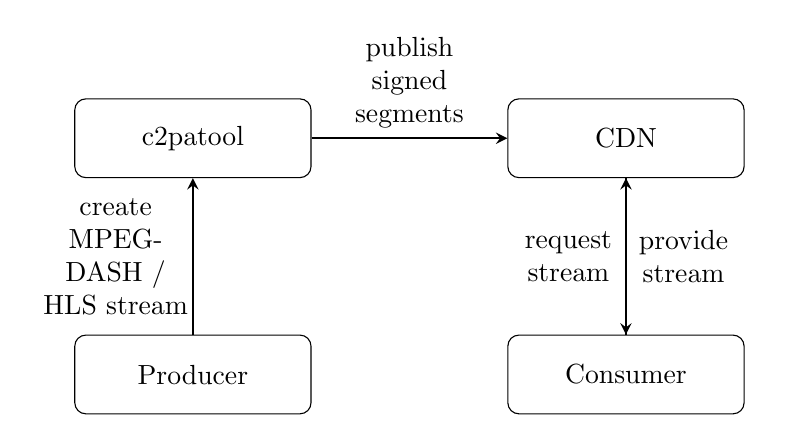
\begin{tikzpicture}[node distance=2cm]
        \node (producer) [component] {Producer};
        \node (c2pa) [component, above of=producer, yshift=1cm] {c2patool};
        \node (cdn) [component, right of=c2pa, xshift=3.5cm] {CDN};
        \node (consumer) [component, below of=cdn, yshift=-1cm] {Consumer};
    
        \draw [arrow] (producer) -- node[anchor=east, text width=2cm, text centered, xshift=0.15cm] {create MPEG-DASH / HLS stream} (c2pa);
        \draw [arrow] (c2pa) -- node[anchor=south, text width=2cm, text centered] {publish signed segments} (cdn);
        \draw [arrow] (consumer) -- node[anchor=east, text width=2cm, text centered, xshift=0.4cm] {request stream} (cdn);
        \draw [arrow] (cdn) -- node[anchor=west, text width=2cm, text centered, xshift=-0.4cm] {provide stream} (consumer);
    \end{tikzpicture}
    \caption{Proof of Concept Testbed Setup}
    \label{fig:setup}
\end{figure}

\section{Challenges}

The challenges to overcome in this task are optimizing the signing process, keeping the added latency and data overhead to as little as possible and figuring out the best method of storing/accessing the C2PA manifest and segment hashes needed for verification.

The problem with the current version of the API that it is only able to sign a complete set of fragmented media segments, i.e. a finished Video-on-Demand (VoD). However, a live stream is continuously generating new media segments, which need to be integrated into the Manifest. That means currently a live streaming testbed would have to sign the entire live stream for every new Segment released and publish it to the CDN. This creates a lot of computational and network overhead.

The Manifest in the Init Segment and each Media Segment contains a hash of its respective file. The Media Segment hashes are used to build a Merkle Tree which enables the verification of a single Segment in the scope of all Segments without requiring to have access to every Segment. Whenever a Segment of the live stream is created this Merkle Tree has to be updated.

My proposal for optimization is to add a new function that takes the Init Segment, output and Signer just like the current API but changes the list of to-be-signed Segments to a list of already-signed Segments and adds a new parameter that is the newly created Segment.

Optimizing the signing process as much as possible should keep the latency overhead to a minimum. No added latency is impossible since a completely new step is added to the production of content. Ideally the encoding, packaging an signing of Media will happen in the same process in the future, allow the added latency in the proposed testbed to be neglected for measurements.

Limiting the data overhead and figuring out the best way to work with the verification data is closely related challenge and also has different possibilities that need to be explored and measured and validated.

One option is to keep the data in the Segments as they are currently. However, one disadvantage of this is that despite the optimized signing process, proposed previously, this still requires that for every new Segment all previously created Segments have to be published to the CDN anew, since a very minute part of their "uuid" Box has changed. The changes are required for verification in the current state of the live stream. Another disadvantage has to do with the verification by the consuming clients. The Init Segment is usually only requested at the very start of the viewing and whenever the client wants to switch to a different streaming quality. However, the Init Segment is constantly changing for every new Segment and that means clients would need to also request the Init Segment with every new Segment they request to get the up-to-date verification data out of them.

One alternative would be to store the Verification data of the Init Segment in the index file, the Media Presentation Description (MPD) file for MPEG-DASH and the Master playlist for HLS. This is a file that contains all the information needed by media players, i.e. \texttt{dash.js} and \texttt{hls.js}, to request the media stream. In the context of live streaming it is not unusual that players refresh said MPD with every new Segment anyways.

One final possibility would be to store the Verification data on a separate server. However, this would add a lot of complexity and new point of attack and failure.

\section{Time Schedule} 

A visual representation of the following schedule is depicted in \Cref{gantt:timeplan}.

I plan on having the proposal to be accepted by the end of January/early February. In the mean time I will begin with the setup of the basic testbed structure. This step will include the creation of an customizable FFmpeg script acting as the Producer, the extension of the \texttt{c2patool} by a CLI flag to make it able to receive an MPEG-DASH and HLS live stream using HTTP and forward segments, the implementation of an HTTP server to act as the CDN and finally a simple webpage that can play the CDN-hosted live stream using \texttt{dash.js} and \texttt{hls.js}. I am expecting this step to take no more than four weeks.

In parallel to the initial setup I will begin writing the first draft of the thesis.

Next, I will conduct a rudimentary experiment to see how this setup forwards with the current state of the API (signing the entire live stream for every new Segment). Using this I will begin the implementation with the verification first, because it is safe to assume that the current API is working correctly and using that I can check if my verification is working. For the verification I will hook into the even listeners of \texttt{dash.js} to inspect the received Segments, parse the C2PA "uuid" Box from the data and then perform the verification in accordance to the specifications. I plan on having this step completed in two to four weeks.

Afterwards, I begin with the optimization of the signing process. I expect this task to be the bulk of the thesis and that this will take up to twelve weeks.

Towards the end of the optimization I will explore the alternative methods of verification in parallel (storing the Verification data in the MPD file and on a separate server) and evaluate all approaches.

I aim to conclude the first draft in conjunction with the evaluation to be able to sync-up with my supervisors to discuss final changes needed to finish the thesis and be able to submit the results by the end of July.

\begin{figure}[t]
    \begin{center}
        \begin{ganttchart}[
            y unit title=0.4cm,
            y unit chart=0.5cm,
            vgrid,hgrid, 
            title label anchor/.style={below=-1.6ex},
            title left shift=.05,
            title right shift=-.05,
            title height=1,
            progress label text={},
            bar height=0.7,
            group right shift=0,
            group top shift=.6,
            group height=.3
        ]{1}{28}
            %labels
            \gantttitle{January}{4} 
            \gantttitle{February}{4} 
            \gantttitle{March}{4} 
            \gantttitle{April}{4} 
            \gantttitle{May}{4} 
            \gantttitle{June}{4}
            \gantttitle{July}{4} \\
            %tasks
            \ganttbar{Proposal}{3}{5} \\
            \ganttbar{Testbed Setup}{5}{8} \\
            \ganttbar{First Draft}{7}{24} \\
            \ganttbar{Experiment}{8}{9} \\
            \ganttbar{Verification}{9}{12} \\
            \ganttbar{Optimize Signing}{12}{23} \\
            \ganttbar{Evaluation}{22}{25} \\
            \ganttbar{Finalize Thesis}{25}{26} \\
            \ganttbar{Submit Thesis}{26}{28}
        \end{ganttchart}
    \end{center}
    \caption{Time Schedule}
    \label{gantt:timeplan}
\end{figure}

\end{document}